%%%%%%%%%%%%%%%%%%%%%%%%
%
% $Autor: Wings $
% $Datum: 2020-07-24 09:05:07Z $
% $Pfad: GDV/Vortraege/latex - Ausarbeitung/Kapitel/Einleitung.tex $
% $Version: 4732 $
%
%%%%%%%%%%%%%%%%%%%%%%%%

\chapter{PortentaH7}
	The PortentaH7 is a high-performance microcontroller board developed by Arduino. It is designed to cater to professional applications, offering robust computing power, advanced features, and versatility. Here are some key aspects of the PortentaH7:
	
	Within the H7 family, there are two variants; H7 Lite and H7 Lite Connected. All the three boards and their differences are presented in this datasheet.
	
	\textbf{Target Areas}: 
	Laboratory equipment, Computer vision
	
	\begin{figure}
		\begin{center}
			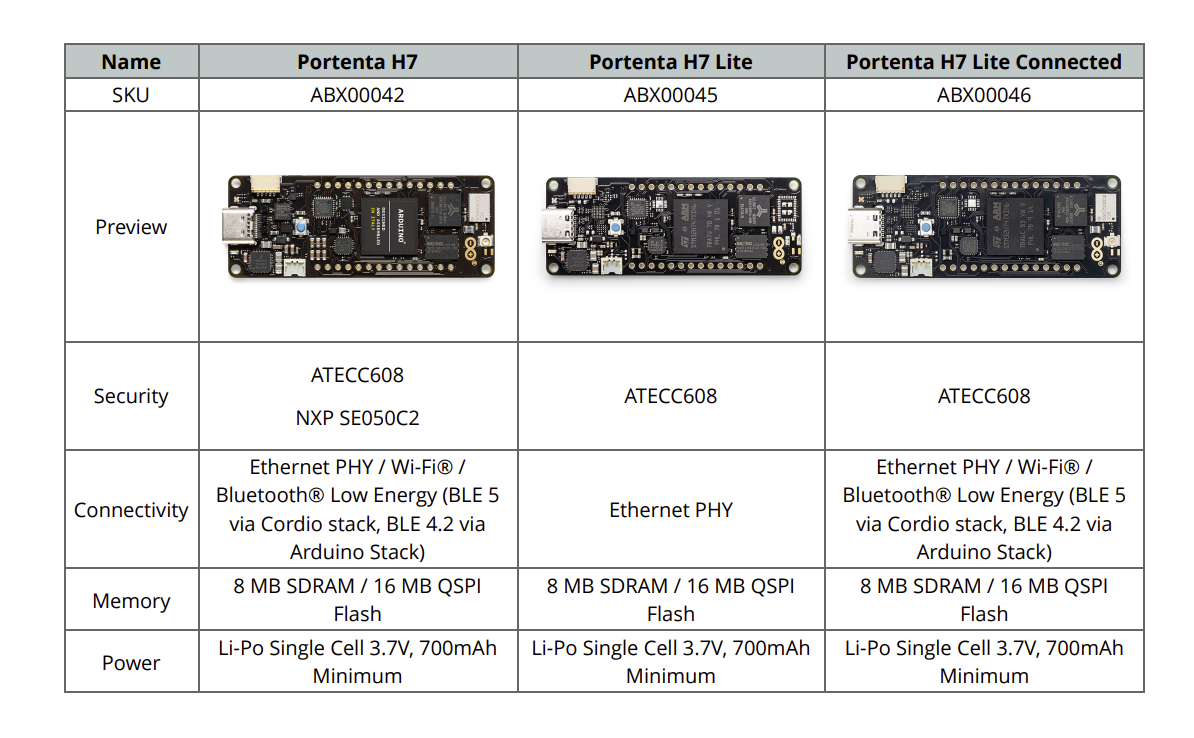
\includegraphics[width=0.7\linewidth]{Images/PortentaH7/TypesofPortentaH7.png}
			\caption{Types of PortentaH7}
			\label{Types}
		\end{center}
	\end{figure}
	
\section{Key Features:}

\textbf{Dual-core Processor:}

\begin{itemize}
	\item Cortex-M7: Runs at up to 480 MHz.
	\item Cortex-M4: Runs at up to 240 MHz.
	\item These cores can operate simultaneously, allowing for efficient parallel processing and real-time application execution.
\end{itemize}

\textbf{Memory:}
\begin{itemize}
	\item RAM: 1 MB of SRAM and 16 MB of SDRAM.
	\item Flash Storage: 8 MB.
\end{itemize}

\textbf{Connectivity:}
\begin{itemize}
	\item $<$ Built-in GPU for handling advanced graphical interfaces. 
	\item $<$ Supports an external display through a dedicated connector.
\end{itemize}

\textbf{Security:}
\begin{itemize}
	\item Hardware cryptography support for secure applications.
	\item Secure boot and secure firmware updates.
\end{itemize}

\textbf{Expansion Options:}
\begin{itemize}
	\item Compatible with Arduino MKR and \textbf{Portenta Vision Shield.}
	\item High-density connectors for custom hardware extensions.
\end{itemize}

\textbf{Operating Systems:}
\begin{itemize}
	\item Capable of running high-level OS like Arm Mbed OS or real-time operating systems (RTOS).
	\item Compatible with Arduino programming environment and libraries.
\end{itemize}

\textbf{Power Management:}
\begin{itemize}
	\item Multiple power supply options: USB-C, Li-Po battery, or external sources.
	\item Low power modes for energy-efficient applications.
\end{itemize}

\textbf{Applications:} \newline
	The Portenta H7 is suitable for a wide range of professional applications, including but not limited to:
\begin{itemize}
	\item \textbf{Industrial IoT:} Real-time monitoring, data acquisition, and control systems.
	\item \textbf{Edge Computing:} Local data processing and decision-making.
	\item \textbf{AI and Machine Learning:} On-device inference and analytics.
	\item \textbf{Robotics:} Advanced motor control and sensor integration.
	\item \textbf{Smart Devices:} Connected appliances, home automation, and wearables.
\end{itemize}

\section{Onboard Sensors with Examples}

	\subsection{Murata 1DX Bluetooth® 5.1}
		The onboard Bluetooth® module of the Portenta H7 offers low energy Bluetooth® functionality, in order to provide the board with the flexibility to be easily connected to devices which also support Bluetooth® Low Energy, such as the Arduino Nano 33 IoT or most modern smartphones. Compared to classic Bluetooth®, Low Energy Bluetooth® is intended to provide considerably reduced power consumption and cost while maintaining a similar communication range. \cite{bluetoothPortentaH7:2024}
		
		\subsubsection{Overview}
			In this Example we will enable low energy Bluetooth® on the Portenta H7 to allow an external Bluetooth® device to control the built-in LED either by turning it on or off.
	
		\subsubsection{Goals}
			\begin{itemize}
				\item Enabling Bluetooth® Low Energy connectivity on the Portenta H7.
				\item Connecting the Portenta to an external Bluetooth® Low Energy Mobile Application (In this case nRF Connect by Nordic Semiconductor).
			\end{itemize}
			
		\subsubsection{Required Hardware and Software}
			\begin{itemize}
				\item Portenta H7 (ABX00042) or Portenta H7 Lite Connected (ABX00046)
				\item USB-C® cable (either USB-A to USB-C® or USB-C® to USB-C®)
				\item Arduino IDE 1.8.13+ or Arduino Pro IDE 0.0.4+
				\item Mobile device, phone or tablet
				\item nRFconnect or equivalent tool downloaded on your mobile device: nRF Connect for iOS or nRF Connect for android
			\end{itemize}
			
		\subsubsection{Instructions}
			\begin{itemize}
				\item \textbf{Configuring the Development Environment:} To communicate with the Portenta H7 via Bluetooth®, you need to upload a pre-built sketch that starts a Bluetooth® network and allows your mobile device, which will be used to control the LEDs, to connect to it. The sketch uses the ArduinoBLE Library that enables the Bluetooth® Low Energy module and handles important functions, such as scanning, connecting and interacting with services provided by other devices. You will also be using a third party application (e.g. nRF Connect), running on your mobile device in order to connect your device to the board and help you control the built-in LED. ~\ref{Bluetooth-portentaH7}
					\begin{figure}
						\begin{center}
							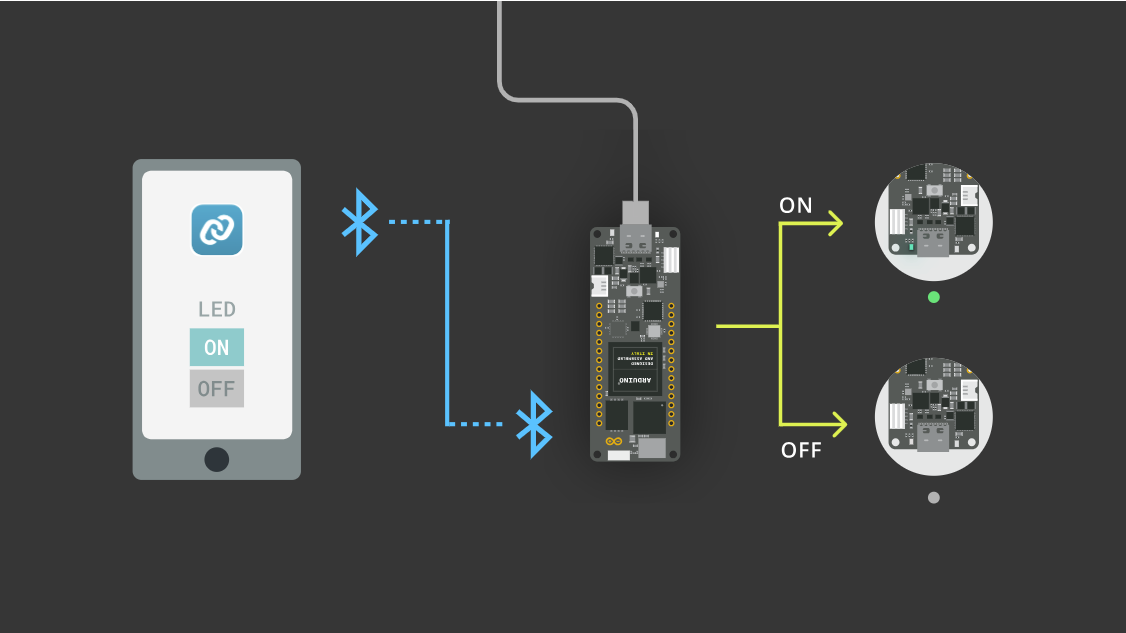
\includegraphics[width=0.7\linewidth]{Images/PortentaH7/Bluetooth-portentaH7.png}
							\caption{Bluetooth-portentaH7}
							\label{Bluetooth-portentaH7}
						\end{center}
					\end{figure}
					
				\item \textbf{1. The Basic Setup:} Begin by plugging in your Portenta board to the computer using a USB-C® cable and open the Arduino IDE. If this is your first time running Arduino sketch files on the board, we suggest you check out how to set up the Portenta H7 for Arduino before you proceed.
					\begin{figure}
						\begin{center}
							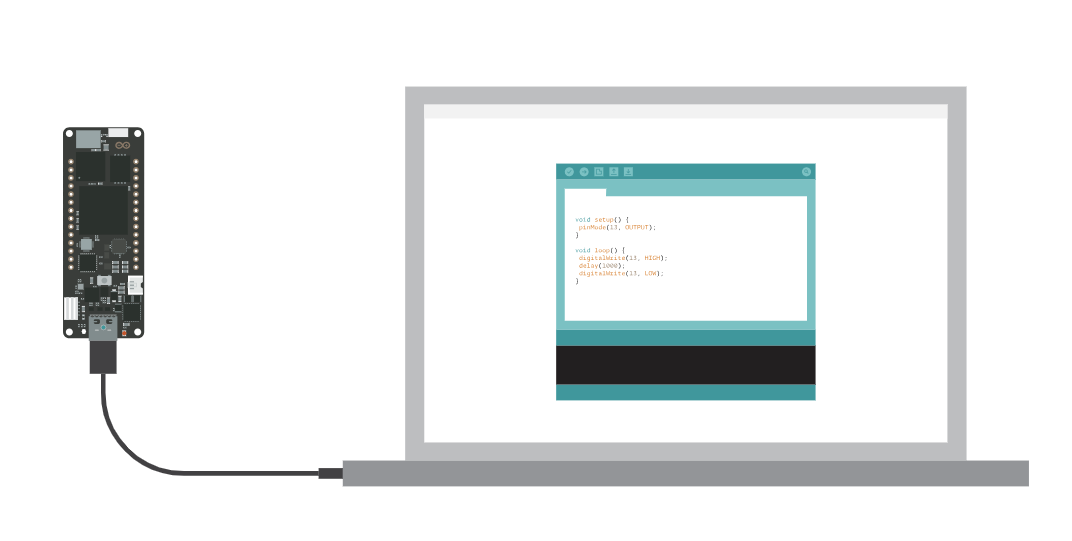
\includegraphics[width=0.7\linewidth]{Images/PortentaH7/PortentaH7-connection.png}
							\caption{PortentaH7-connection}
							\label{PortentaH7-connection}
						\end{center}
					\end{figure}
				
				\item \textbf{2. Install the ArduinoBLE Library:} You will need to install the ArduinoBLE library in the Arduino IDE you are using. To install the library go to : Tools > Manage Libraries... type ArduinoBLE and click Install. Make sure you install ArduinoBLE version 1.1.3 or higher. ~\ref{Bluetooth-Library}
					\begin{figure}
						\begin{center}
							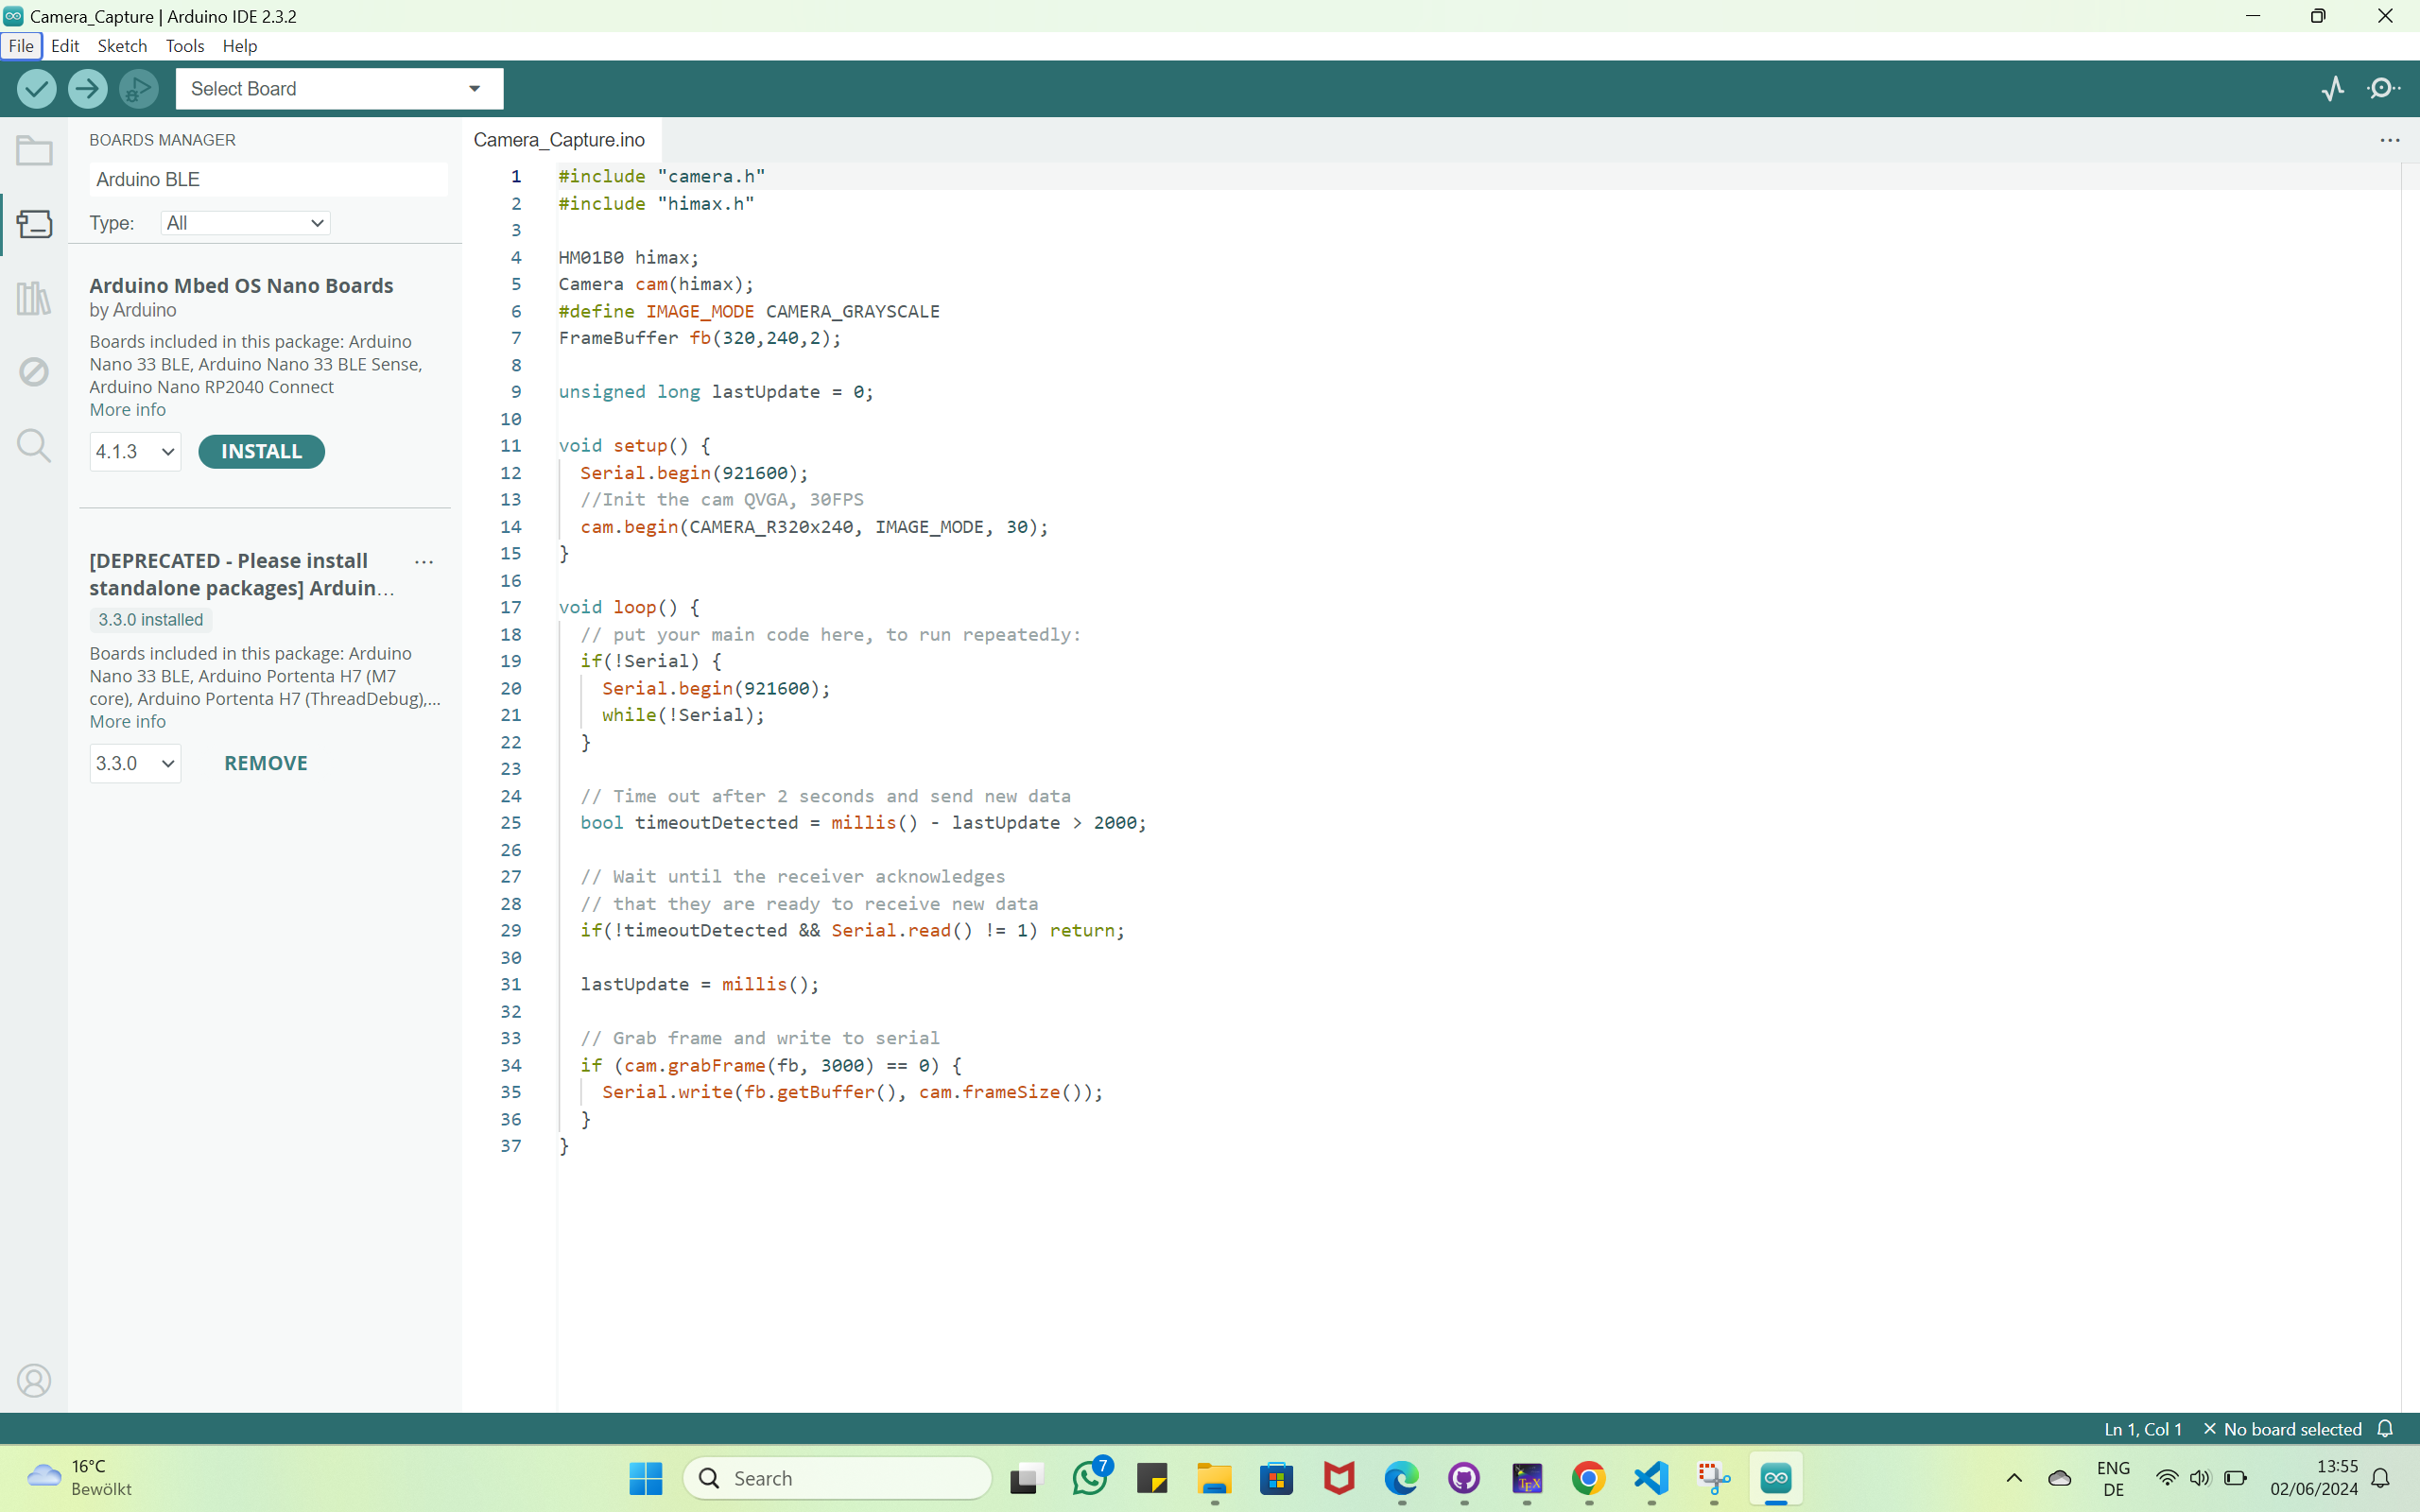
\includegraphics[width=0.7\linewidth]{Images/PortentaH7/Bluetooth-Library.png}
							\caption{Bluetooth-Library}
							\label{Bluetooth-Library}
						\end{center}
					\end{figure}
				
				\item \textbf{3. Create the Bluetooth® Low Energy Sketch:} Let's program the Portenta with the following example sketch. If the Bluetooth® Low Energy module has been initialized correctly, you will see the blue LED lighting up for one second after uploading the sketch. If it fails, you will see the red LED lighting up instead. Copy and paste the following code into a new sketch in your IDE or download it from Arduino-Pro-Tutorials in the Arduino IDE and open it from: Examples > Arduino-Pro-Tutorials > BLE Connectivity on Portenta H7 > PortentaBLE 
					\begin{lstlisting}
						#include <ArduinoBLE.h>
						
						BLEService ledService("19b10000-e8f2-537e-4f6c-d104768a1214");
						
						// Bluetooth Low Energy LED Switch Characteristic - custom 128-bit UUID, read and writable by central
						BLEByteCharacteristic switchCharacteristic("19b10000-e8f2-537e-4f6c-d104768a1214", BLERead | BLEWrite);
						
						const int ledPin = LED-BUILTIN; // Pin to use for the LED
						
						void setup() {
							Serial.begin(9600);
							//while (!Serial);   // Uncomment to wait for serial port to connect.
							
							// Set LED pin to output mode
							pinMode(ledPin, OUTPUT);
							digitalWrite(ledPin, HIGH);
							
							// Begin initialization
							if (!BLE.begin()) {
								Serial.println("Starting Bluetooth Low Energy failed!");
								digitalWrite(LEDR, LOW);
								delay(1000);
								digitalWrite(LEDR, HIGH);
								
								// Stop if Bluetooth Low Energy couldn't be initialized.
								while (1);
							}
							
							// Set advertised local name and service UUID:
							BLE.setLocalName("LED-Portenta-01");
							BLE.setAdvertisedService(ledService);
							
							// Add the characteristic to the service
							ledService.addCharacteristic(switchCharacteristic);
							
							// Add service
							BLE.addService(ledService);
							
							// Set the initial value for the characeristic:
							switchCharacteristic.writeValue(0);
							
							// start advertising
							BLE.advertise();
							digitalWrite(LEDB, LOW);
							delay(1000);
							digitalWrite(LEDB, HIGH);
							Serial.println("BLE LED Control ready");
						}
						
						void loop() {
							// Listen for Bluetooth Low Energy peripherals to connect:
							BLEDevice central = BLE.central();
							
							// If a central is connected to peripheral:
							if (central) {
								Serial.print("Connected to central: ");
								// Print the central's MAC address:
								Serial.println(central.address());
								digitalWrite(LEDB, HIGH);
								delay(100);
								digitalWrite(LEDB, LOW);
								delay(100);
								digitalWrite(LEDB, HIGH);
								
								// While the central is still connected to peripheral:
								while (central.connected()) {
									// If the remote device wrote to the characteristic,
									// Use the value to control the LED:
									if (switchCharacteristic.written()) {
										if (switchCharacteristic.value()) {   // Any value other than 0
											Serial.println("LED on");
											digitalWrite(ledPin, LOW);          // Will turn the Portenta LED on
										} else {                             
											Serial.println("LED off");
											digitalWrite(ledPin, HIGH);         // Will turn the Portenta LED off          
										}
									}
								}
								
								// When the central disconnects, print it out:
								Serial.print("Disconnected from central: ");
								Serial.println(central.address());    
								digitalWrite(LEDB, HIGH);
								delay(100);
								digitalWrite(LEDB, LOW);
								delay(100);
								digitalWrite(LEDB, HIGH);
							}
						}    
								
					\end{lstlisting}
					
					In this example, you use a pre-defined Bluetooth number code pre-setup for controlling a device's LED. This code can also be referred to as GATT codes, which define how two Bluetooth® low energy devices transfer data. Once a connection is established with a device, its respective GATT code, which is a 16 bit identifier, is stored in a lookup table for future reference.
					
					These GATT codes are very long, but, in this example, it is always the same code:
					\begin{lstlisting}
						BLEService ledService("19b10000-e8f2-537e-4f6c-d104768a1214"); // BLE LED Service
					\end{lstlisting}	
					
				\item \textbf{4. Upload the Sketch:} Double press the reset button so the built-in LED is slowly pulsing green. Then, select your board in the menu: Tools > Board > Arduino Portenta H7 (M7 core) ~\ref{select-board-h7}
					\begin{figure}
						\begin{center}
							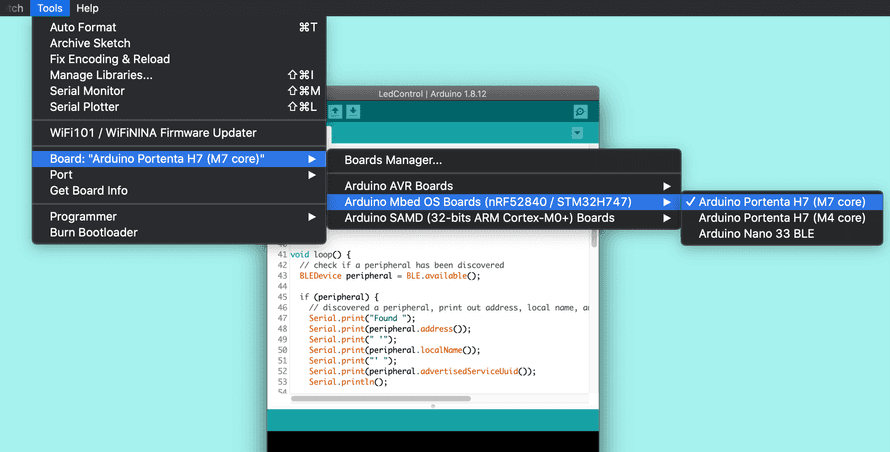
\includegraphics[width=0.7\linewidth]{Images/PortentaH7/select-board-h7.png}
							\caption{select-board-h7}
							\label{select-board-h7}
						\end{center}
					\end{figure}
					
				Choose the Port where your Portenta is connected to and Upload the sketch. Open the Serial Monitor once you have uploaded the code to the board to see debugging messages. If the Bluetooth® Low Energy setup was successful, you should see the message BLE LED Control ready. If something went wrong, you will see the message Starting Bluetooth® Low Energy failed!. In that case update the Arduino BLE library (in the Library Manager) and the board (in the Board Manager) to the latest version and try again. ~\ref{select-port}
				
					\begin{figure}
						\begin{center}
							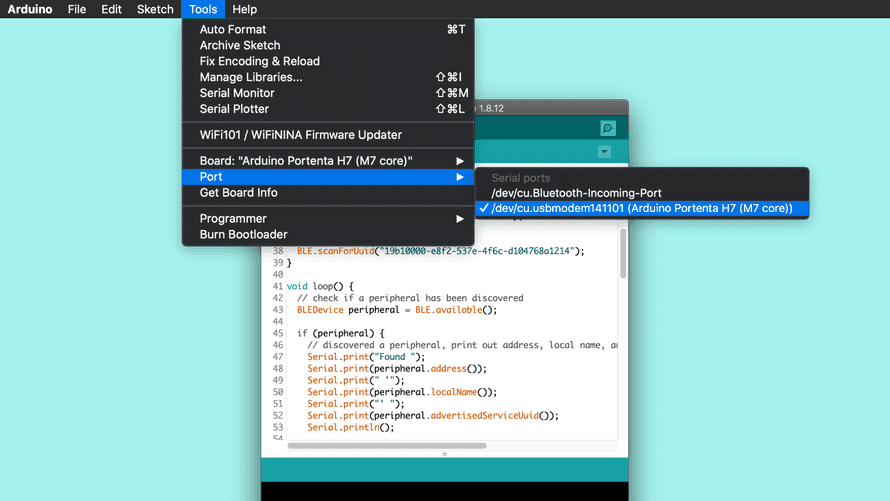
\includegraphics[width=0.7\linewidth]{Images/PortentaH7/select-port.png}
							\caption{select-port}
							\label{select-port}
						\end{center}
					\end{figure}
					
				\item \textbf{5.  Connect an External Device :} On your mobile device install nRF Connect or an equivalent app that allows for Bluetooth® Low Energy connections. We will refer to nRF Connect for the rest of this tutorial. ~\ref{NRF-Connect}
					\begin{figure}
						\begin{center}
							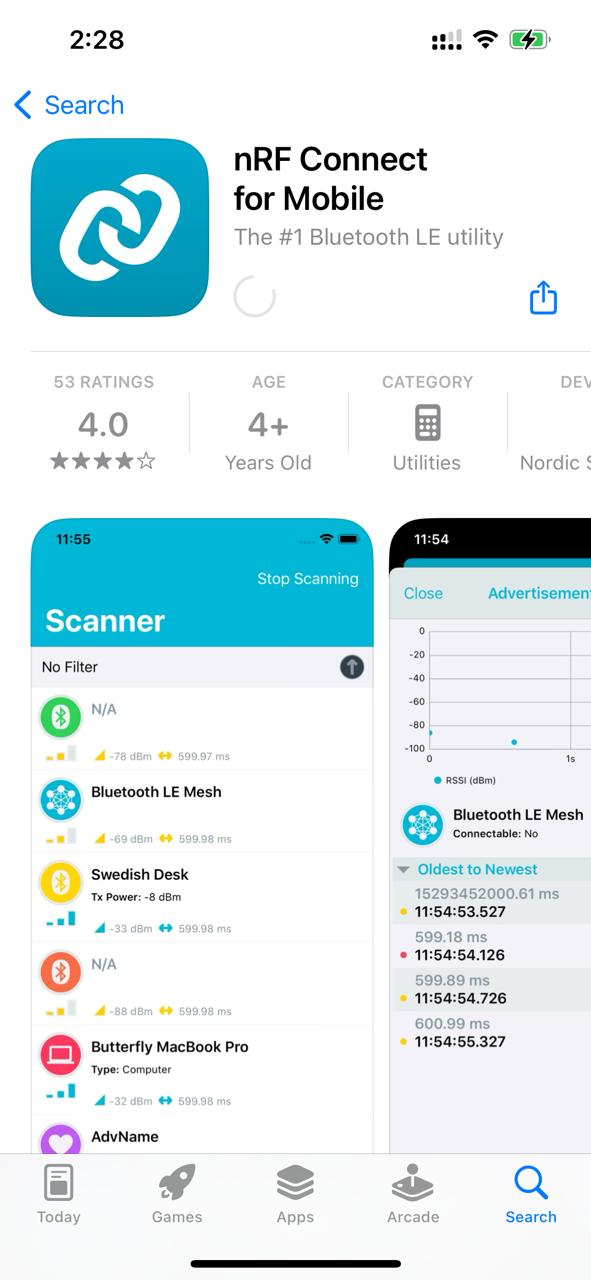
\includegraphics[width=0.7\linewidth]{Images/PortentaH7/NRF-Connect.jpg}
							\caption{NRF-Connect}
							\label{NRF-Connect}
						\end{center}
					\end{figure}
				Once you have downloaded the nRF application on your mobile device, look for your Portenta in the device list. You may filter the list by "Portenta" to easierly find your board in case you are using nRF Connect.
				
				\item When you find your board in the list tap "Connect".
				\item Navigate to the "Services" screen and tap the arrow up button.
				\item Switch to "Bool" type and move the toggle to "True". Confirm the dialog with a tap on "Write" and you should see the built-in LED turned on. If you do the same procedure again but setting the toggle switch to "False", it will turn off the LED. ~\ref{Bluetooth-scan}
					\begin{figure}
						\begin{center}
							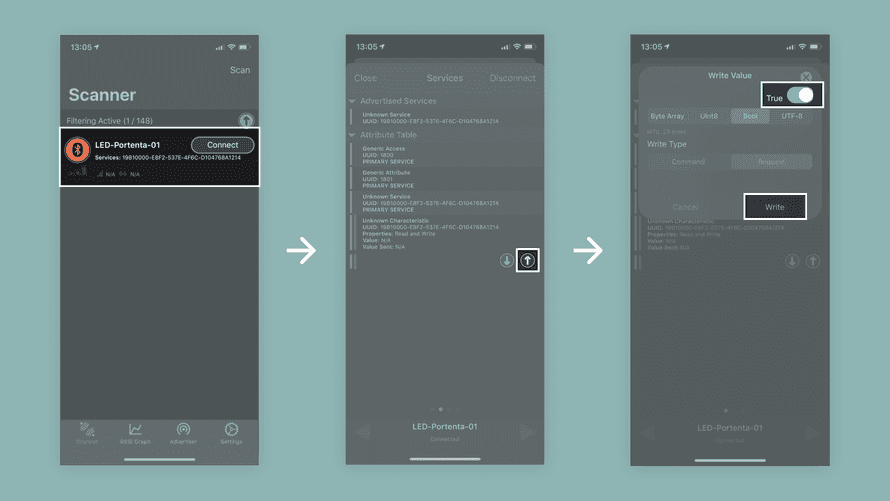
\includegraphics[width=0.7\linewidth]{Images/PortentaH7/Bluetooth-scan.png}
							\caption{Bluetooth-scan}
							\label{Bluetooth-scan}
						\end{center}
					\end{figure}
				\item \textbf{6. Conclusion:} This example shows how to connect and control the built-in LED using a Bluetooth® Low Energy connection. You have learned how a simple Bluetooth® Low Energy connection between your Portenta and your cell phone, which has basic communication abilities between the two devices, works. ~\ref{NRF-Connect}	
				
			\end{itemize}
		

		



\section{First Step with PortentaH7:}
	
	\subsection{Setting Up Portenta H7 For Arduino:}
		This Example teaches you how to set up the board, how to configure your computer and how to run the classic Arduino blink example to verify if the configuration was successful. ~\ref{PortentaH7-connection} \cite{portentaSetup:2024}
	\subsection{Goals:}
		\begin{itemize}
			\item About the Arduino and Mbed operating system (Mbed OS) stack
			\item Installing the Mbed library
			\item Controlling the built in LED on the Portenta board
		\end{itemize}
	\subsection{Instructions:}
		\begin{itemize}
			\item \textbf{Configuring the Development Environment:} In this section, we will guide you through a step-by-step process of setting up your Portenta board for running an Arduino Sketch that blinks the built-in RGB LED.
			\item \textbf{The Basic Setup:} Let's begin by Plug-in your Portenta to your computer using the appropriate USB-C® cable. Next, open your IDE and make sure that you have the right version of the Arduino IDE downloaded on to your computer.
				\begin{figure}
					\begin{center}
						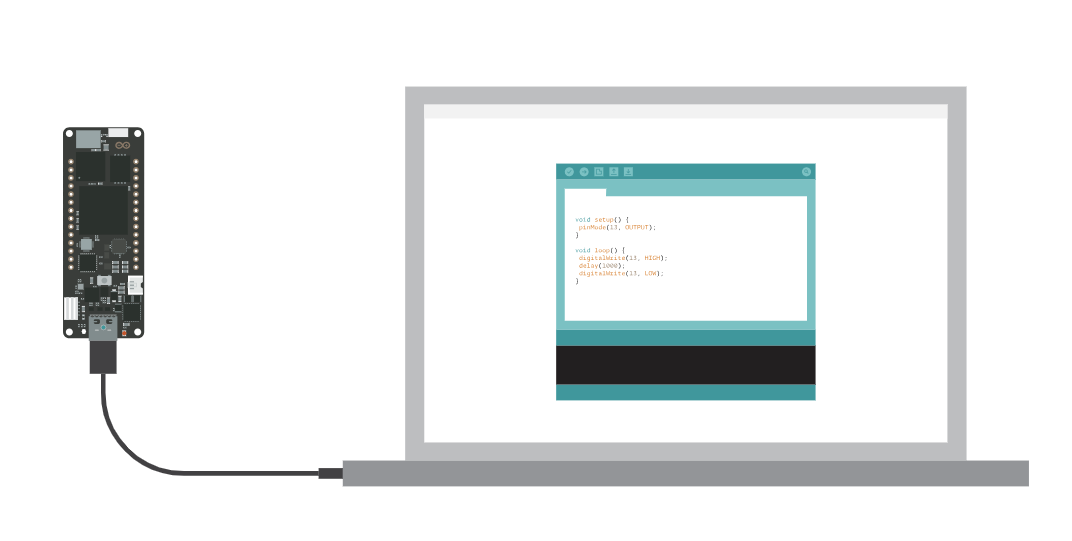
\includegraphics[width=0.7\linewidth]{Images/PortentaH7/PortentaH7-connection.png}
						\caption{PortentaH7-connection}
						\label{PortentaH7-connection}
					\end{center}
				\end{figure}
			\item \textbf{Adding the Portenta to the List of Available Boards:} In your Arduino IDE, open the board manager and search for "portenta". Find the Arduino mbed-enabled Boards library and click on "Install" to install the latest version of the mbed core (1.2.3 at the time of writing this tutorial). ~\ref{Portentaport}
				\begin{figure}
					\begin{center}
						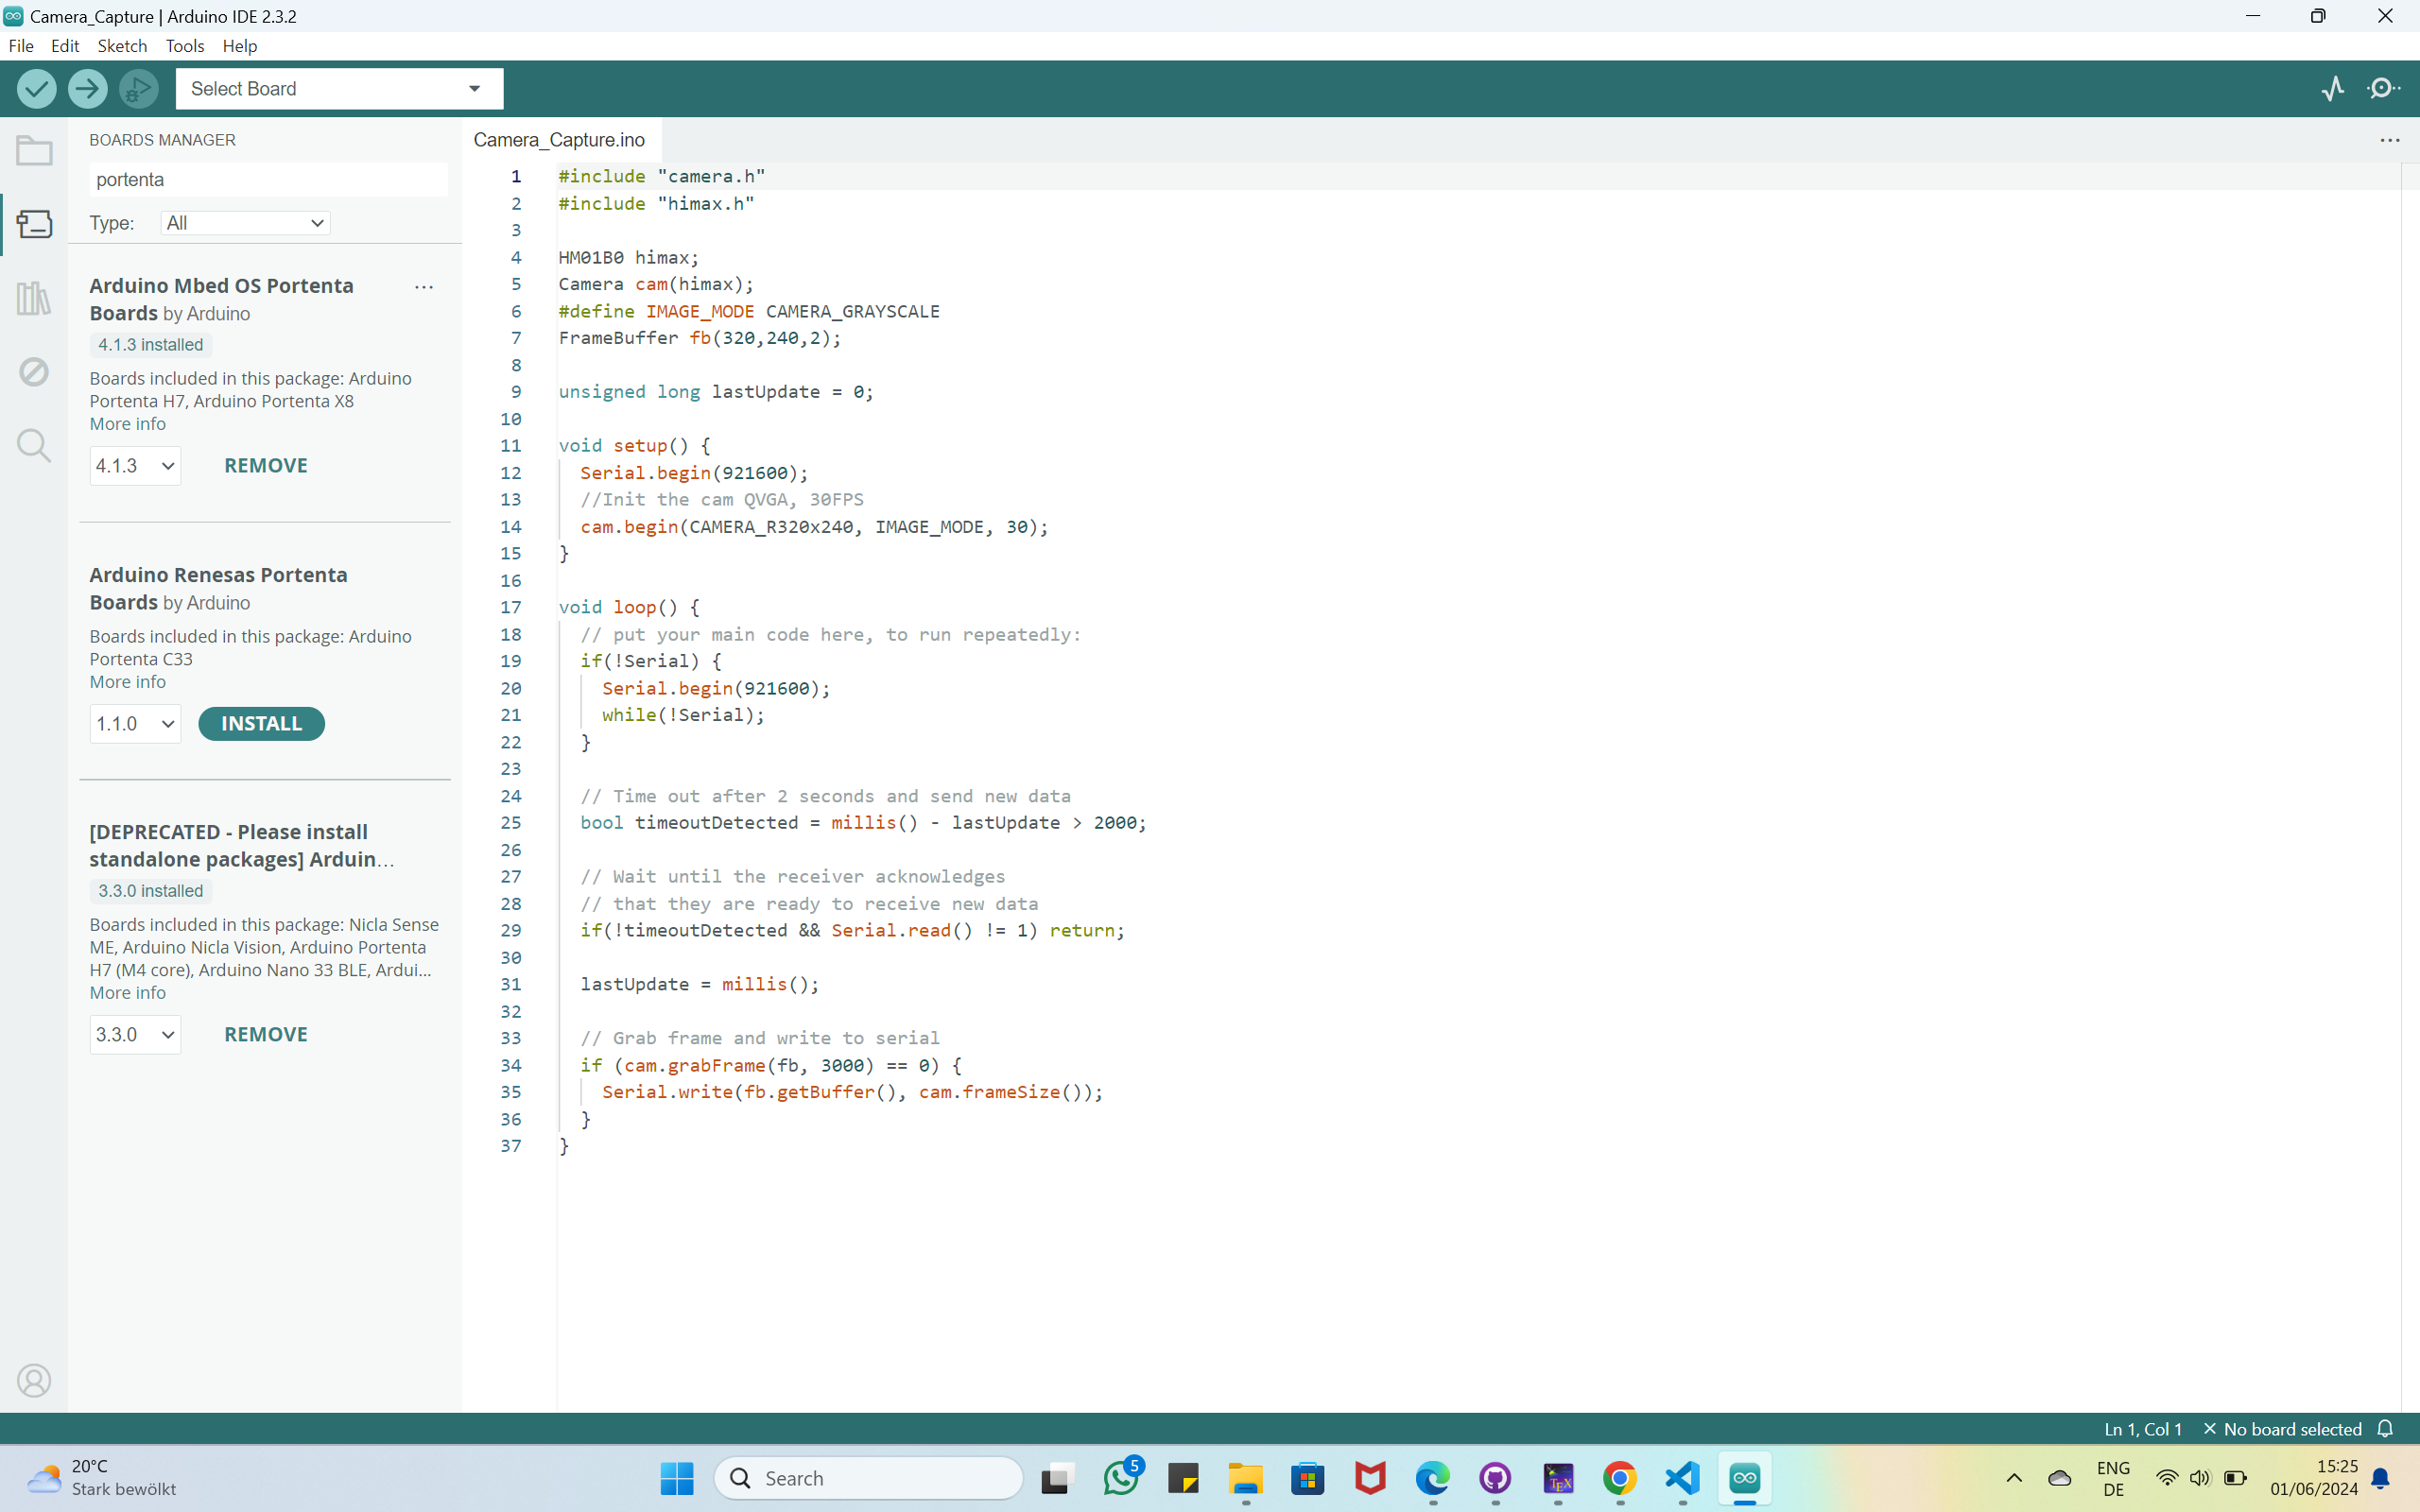
\includegraphics[width=0.7\linewidth]{Images/PortentaH7/Portentaport.png}
						\caption{Portentaport}
						\label{Portentaport}
					\end{center}
				\end{figure}
				
			\item \textbf{Uploading the Classic Blink Sketch:} Let's program the Portenta with the classic blink example to check if the connection to the board works. 
			
					\begin{lstlisting}
						// the setup function runs once when you press reset or power the board
						void setup() {
							// initialize digital pin LED_BUILTIN as an output.
							pinMode(LED_BUILTIN, OUTPUT);
							digitalWrite(LED_BUILTIN, HIGH); // turn the LED off after being turned on by pinMode()
						}
						
						// the loop function runs over and over again forever
						void loop() {
							digitalWrite(LED_BUILTIN, LOW); // turn the LED on (LOW is the voltage level)
							delay(1000); // wait for a second
							digitalWrite(LED_BUILTIN, HIGH); // turn the LED off by making the voltage HIGH
							delay(1000); // wait for a second
						}   
								
					\end{lstlisting}
			
		\end{itemize}
		
	\subsection{Conclusion:}
		You have now configured your Portenta board to run Arduino sketches. Along with that you gained an understanding of how the Arduino Core runs on top of Mbed OS.
		
		


	
=======
%%%%%%%%%%%%%%%%%%%%%%%%
%
% $Autor: Wings $
% $Datum: 2020-07-24 09:05:07Z $
% $Pfad: GDV/Vortraege/latex - Ausarbeitung/Kapitel/Einleitung.tex $
% $Version: 4732 $
%
%%%%%%%%%%%%%%%%%%%%%%%%

\chapter{PortentaH7}
	The PortentaH7 is a high-performance microcontroller board developed by Arduino. It is designed to cater to professional applications, offering robust computing power, advanced features, and versatility. Here are some key aspects of the PortentaH7:
	
	Within the H7 family, there are two variants; H7 Lite and H7 Lite Connected. All the three boards and their differences are presented in this datasheet.
	
	\textbf{Target Areas}: 
	Laboratory equipment, Computer vision
	
	\begin{figure}
		\begin{center}
			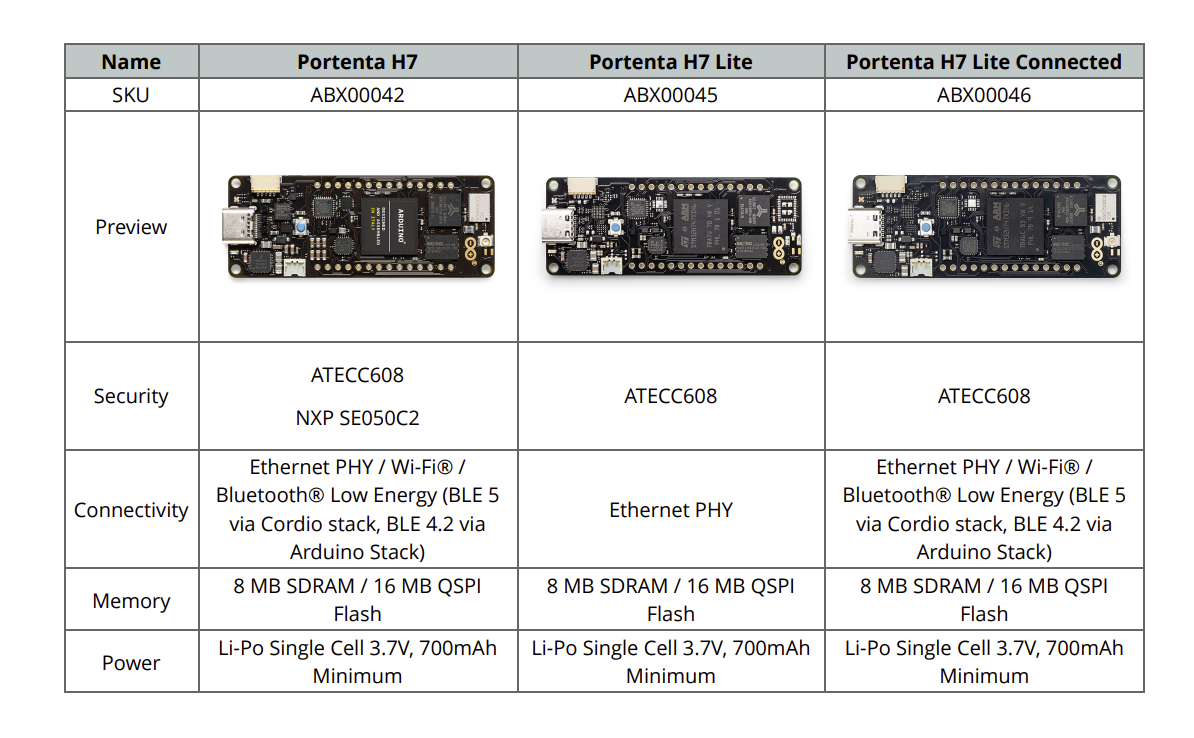
\includegraphics[width=0.7\linewidth]{Images/PortentaH7/TypesofPortentaH7.png}
			\caption{Types of PortentaH7}
			\label{Types}
		\end{center}
	\end{figure}
	
\section{Key Features:}

\textbf{Dual-core Processor:}

\begin{itemize}
	\item Cortex-M7: Runs at up to 480 MHz.
	\item Cortex-M4: Runs at up to 240 MHz.
	\item These cores can operate simultaneously, allowing for efficient parallel processing and real-time application execution.
\end{itemize}

\textbf{Memory:}
\begin{itemize}
	\item RAM: 1 MB of SRAM and 16 MB of SDRAM.
	\item Flash Storage: 8 MB.
\end{itemize}

\textbf{Connectivity:}
\begin{itemize}
	\item $<$ Built-in GPU for handling advanced graphical interfaces. 
	\item $<$ Supports an external display through a dedicated connector.
\end{itemize}

\textbf{Security:}
\begin{itemize}
	\item Hardware cryptography support for secure applications.
	\item Secure boot and secure firmware updates.
\end{itemize}

\textbf{Expansion Options:}
\begin{itemize}
	\item Compatible with Arduino MKR and \textbf{Portenta Vision Shield.}
	\item High-density connectors for custom hardware extensions.
\end{itemize}

\textbf{Operating Systems:}
\begin{itemize}
	\item Capable of running high-level OS like Arm Mbed OS or real-time operating systems (RTOS).
	\item Compatible with Arduino programming environment and libraries.
\end{itemize}

\textbf{Power Management:}
\begin{itemize}
	\item Multiple power supply options: USB-C, Li-Po battery, or external sources.
	\item Low power modes for energy-efficient applications.
\end{itemize}

\textbf{Applications:} \newline
	The Portenta H7 is suitable for a wide range of professional applications, including but not limited to:
\begin{itemize}
	\item \textbf{Industrial IoT:} Real-time monitoring, data acquisition, and control systems.
	\item \textbf{Edge Computing:} Local data processing and decision-making.
	\item \textbf{AI and Machine Learning:} On-device inference and analytics.
	\item \textbf{Robotics:} Advanced motor control and sensor integration.
	\item \textbf{Smart Devices:} Connected appliances, home automation, and wearables.
\end{itemize}

\section{Onboard Sensors with Examples}

	\subsection{Murata 1DX Bluetooth® 5.1}
		The onboard Bluetooth® module of the Portenta H7 offers low energy Bluetooth® functionality, in order to provide the board with the flexibility to be easily connected to devices which also support Bluetooth® Low Energy, such as the Arduino Nano 33 IoT or most modern smartphones. Compared to classic Bluetooth®, Low Energy Bluetooth® is intended to provide considerably reduced power consumption and cost while maintaining a similar communication range. \cite{bluetoothPortentaH7:2024}
		
		\subsubsection{Overview}
			In this Example we will enable low energy Bluetooth® on the Portenta H7 to allow an external Bluetooth® device to control the built-in LED either by turning it on or off.
	
		\subsubsection{Goals}
			\begin{itemize}
				\item Enabling Bluetooth® Low Energy connectivity on the Portenta H7.
				\item Connecting the Portenta to an external Bluetooth® Low Energy Mobile Application (In this case nRF Connect by Nordic Semiconductor).
			\end{itemize}
			
		\subsubsection{Required Hardware and Software}
			\begin{itemize}
				\item Portenta H7 (ABX00042) or Portenta H7 Lite Connected (ABX00046)
				\item USB-C® cable (either USB-A to USB-C® or USB-C® to USB-C®)
				\item Arduino IDE 1.8.13+ or Arduino Pro IDE 0.0.4+
				\item Mobile device, phone or tablet
				\item nRFconnect or equivalent tool downloaded on your mobile device: nRF Connect for iOS or nRF Connect for android
			\end{itemize}
			
		\subsubsection{Instructions}
			\begin{itemize}
				\item \textbf{Configuring the Development Environment:} To communicate with the Portenta H7 via Bluetooth®, you need to upload a pre-built sketch that starts a Bluetooth® network and allows your mobile device, which will be used to control the LEDs, to connect to it. The sketch uses the ArduinoBLE Library that enables the Bluetooth® Low Energy module and handles important functions, such as scanning, connecting and interacting with services provided by other devices. You will also be using a third party application (e.g. nRF Connect), running on your mobile device in order to connect your device to the board and help you control the built-in LED. ~\ref{Bluetooth-portentaH7}
					\begin{figure}
						\begin{center}
							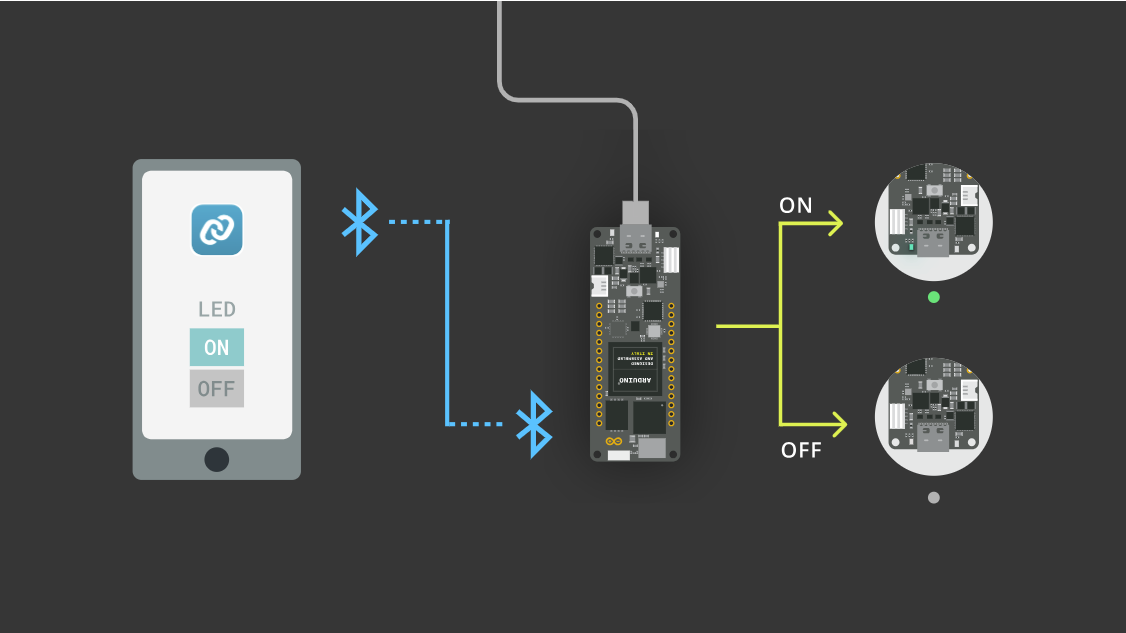
\includegraphics[width=0.7\linewidth]{Images/PortentaH7/Bluetooth-portentaH7.png}
							\caption{Bluetooth-portentaH7}
							\label{Bluetooth-portentaH7}
						\end{center}
					\end{figure}
					
				\item \textbf{1. The Basic Setup:} Begin by plugging in your Portenta board to the computer using a USB-C® cable and open the Arduino IDE. If this is your first time running Arduino sketch files on the board, we suggest you check out how to set up the Portenta H7 for Arduino before you proceed.
					\begin{figure}
						\begin{center}
							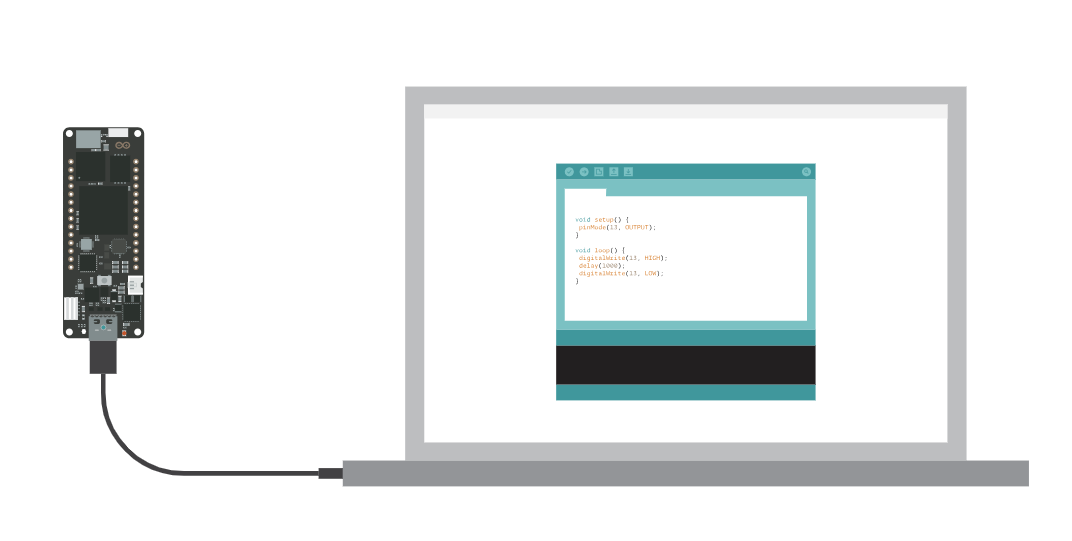
\includegraphics[width=0.7\linewidth]{Images/PortentaH7/PortentaH7-connection.png}
							\caption{PortentaH7-connection}
							\label{PortentaH7-connection}
						\end{center}
					\end{figure}
				
				\item \textbf{2. Install the ArduinoBLE Library:} You will need to install the ArduinoBLE library in the Arduino IDE you are using. To install the library go to : Tools > Manage Libraries... type ArduinoBLE and click Install. Make sure you install ArduinoBLE version 1.1.3 or higher. ~\ref{Bluetooth-Library}
					\begin{figure}
						\begin{center}
							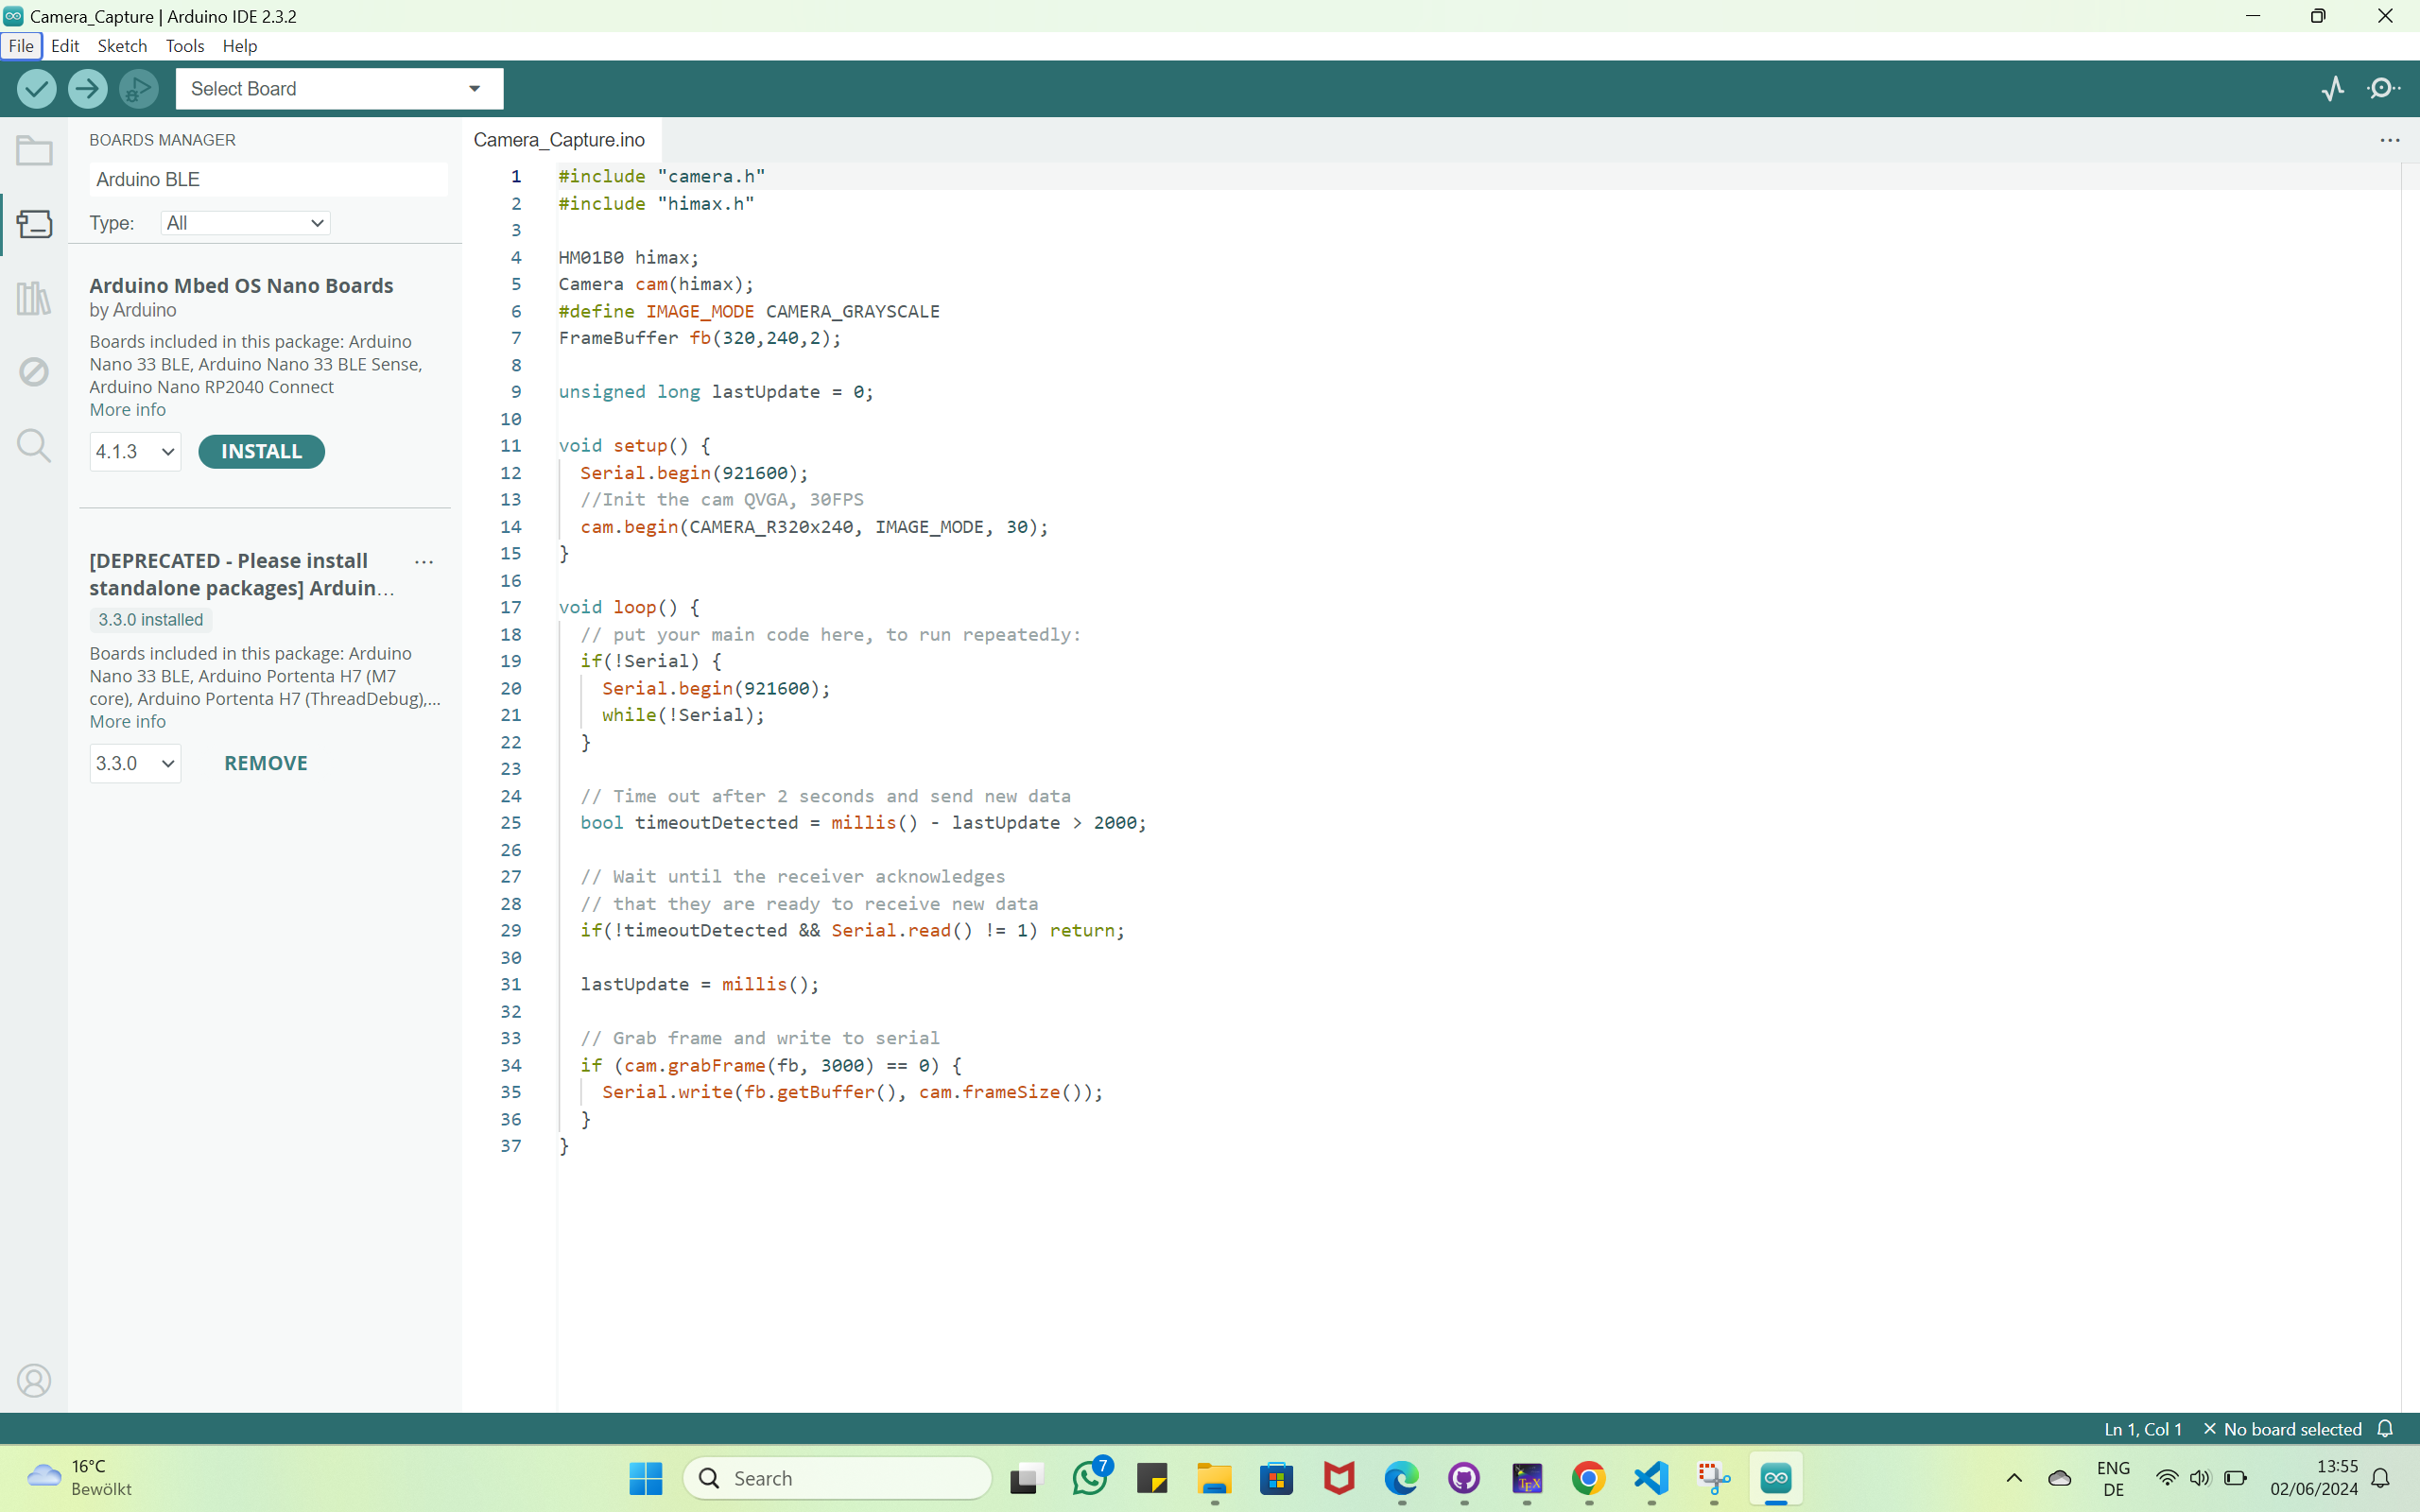
\includegraphics[width=0.7\linewidth]{Images/PortentaH7/Bluetooth-Library.png}
							\caption{Bluetooth-Library}
							\label{Bluetooth-Library}
						\end{center}
					\end{figure}
				
				\item \textbf{3. Create the Bluetooth® Low Energy Sketch:} Let's program the Portenta with the following example sketch. If the Bluetooth® Low Energy module has been initialized correctly, you will see the blue LED lighting up for one second after uploading the sketch. If it fails, you will see the red LED lighting up instead. Copy and paste the following code into a new sketch in your IDE or download it from Arduino-Pro-Tutorials in the Arduino IDE and open it from: Examples > Arduino-Pro-Tutorials > BLE Connectivity on Portenta H7 > PortentaBLE 
					\begin{lstlisting}
						#include <ArduinoBLE.h>
						
						BLEService ledService("19b10000-e8f2-537e-4f6c-d104768a1214");
						
						// Bluetooth Low Energy LED Switch Characteristic - custom 128-bit UUID, read and writable by central
						BLEByteCharacteristic switchCharacteristic("19b10000-e8f2-537e-4f6c-d104768a1214", BLERead | BLEWrite);
						
						const int ledPin = LED-BUILTIN; // Pin to use for the LED
						
						void setup() {
							Serial.begin(9600);
							//while (!Serial);   // Uncomment to wait for serial port to connect.
							
							// Set LED pin to output mode
							pinMode(ledPin, OUTPUT);
							digitalWrite(ledPin, HIGH);
							
							// Begin initialization
							if (!BLE.begin()) {
								Serial.println("Starting Bluetooth Low Energy failed!");
								digitalWrite(LEDR, LOW);
								delay(1000);
								digitalWrite(LEDR, HIGH);
								
								// Stop if Bluetooth Low Energy couldn't be initialized.
								while (1);
							}
							
							// Set advertised local name and service UUID:
							BLE.setLocalName("LED-Portenta-01");
							BLE.setAdvertisedService(ledService);
							
							// Add the characteristic to the service
							ledService.addCharacteristic(switchCharacteristic);
							
							// Add service
							BLE.addService(ledService);
							
							// Set the initial value for the characeristic:
							switchCharacteristic.writeValue(0);
							
							// start advertising
							BLE.advertise();
							digitalWrite(LEDB, LOW);
							delay(1000);
							digitalWrite(LEDB, HIGH);
							Serial.println("BLE LED Control ready");
						}
						
						void loop() {
							// Listen for Bluetooth Low Energy peripherals to connect:
							BLEDevice central = BLE.central();
							
							// If a central is connected to peripheral:
							if (central) {
								Serial.print("Connected to central: ");
								// Print the central's MAC address:
								Serial.println(central.address());
								digitalWrite(LEDB, HIGH);
								delay(100);
								digitalWrite(LEDB, LOW);
								delay(100);
								digitalWrite(LEDB, HIGH);
								
								// While the central is still connected to peripheral:
								while (central.connected()) {
									// If the remote device wrote to the characteristic,
									// Use the value to control the LED:
									if (switchCharacteristic.written()) {
										if (switchCharacteristic.value()) {   // Any value other than 0
											Serial.println("LED on");
											digitalWrite(ledPin, LOW);          // Will turn the Portenta LED on
										} else {                             
											Serial.println("LED off");
											digitalWrite(ledPin, HIGH);         // Will turn the Portenta LED off          
										}
									}
								}
								
								// When the central disconnects, print it out:
								Serial.print("Disconnected from central: ");
								Serial.println(central.address());    
								digitalWrite(LEDB, HIGH);
								delay(100);
								digitalWrite(LEDB, LOW);
								delay(100);
								digitalWrite(LEDB, HIGH);
							}
						}    
								
					\end{lstlisting}
					
					In this example, you use a pre-defined Bluetooth number code pre-setup for controlling a device's LED. This code can also be referred to as GATT codes, which define how two Bluetooth® low energy devices transfer data. Once a connection is established with a device, its respective GATT code, which is a 16 bit identifier, is stored in a lookup table for future reference.
					
					These GATT codes are very long, but, in this example, it is always the same code:
					\begin{lstlisting}
						BLEService ledService("19b10000-e8f2-537e-4f6c-d104768a1214"); // BLE LED Service
					\end{lstlisting}	
					
				\item \textbf{4. Upload the Sketch:} Double press the reset button so the built-in LED is slowly pulsing green. Then, select your board in the menu: Tools > Board > Arduino Portenta H7 (M7 core) ~\ref{select-board-h7}
					\begin{figure}
						\begin{center}
							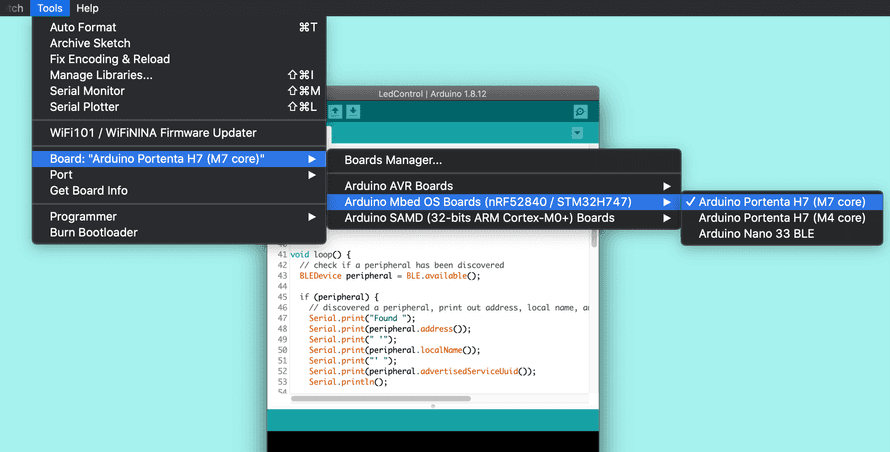
\includegraphics[width=0.7\linewidth]{Images/PortentaH7/select-board-h7.png}
							\caption{select-board-h7}
							\label{select-board-h7}
						\end{center}
					\end{figure}
					
				Choose the Port where your Portenta is connected to and Upload the sketch. Open the Serial Monitor once you have uploaded the code to the board to see debugging messages. If the Bluetooth® Low Energy setup was successful, you should see the message BLE LED Control ready. If something went wrong, you will see the message Starting Bluetooth® Low Energy failed!. In that case update the Arduino BLE library (in the Library Manager) and the board (in the Board Manager) to the latest version and try again. ~\ref{select-port}
				
					\begin{figure}
						\begin{center}
							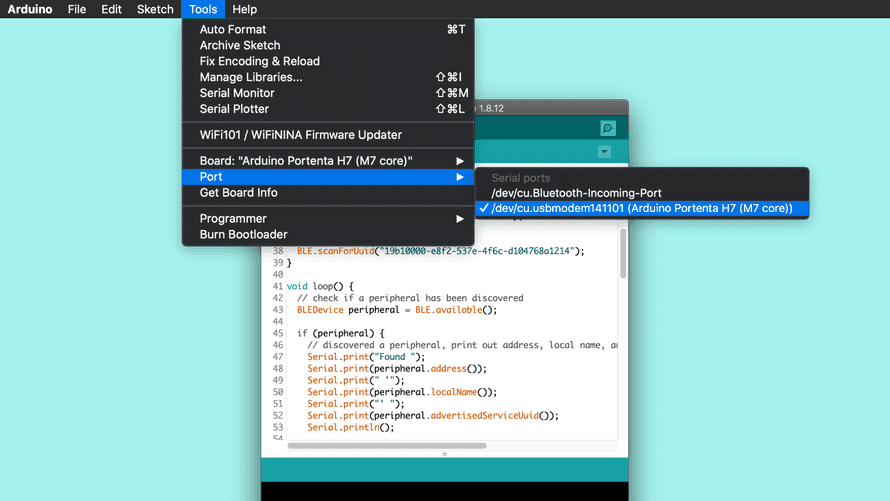
\includegraphics[width=0.7\linewidth]{Images/PortentaH7/select-port.png}
							\caption{select-port}
							\label{select-port}
						\end{center}
					\end{figure}
					
				\item \textbf{5.  Connect an External Device :} On your mobile device install nRF Connect or an equivalent app that allows for Bluetooth® Low Energy connections. We will refer to nRF Connect for the rest of this tutorial. ~\ref{NRF-Connect}
					\begin{figure}
						\begin{center}
							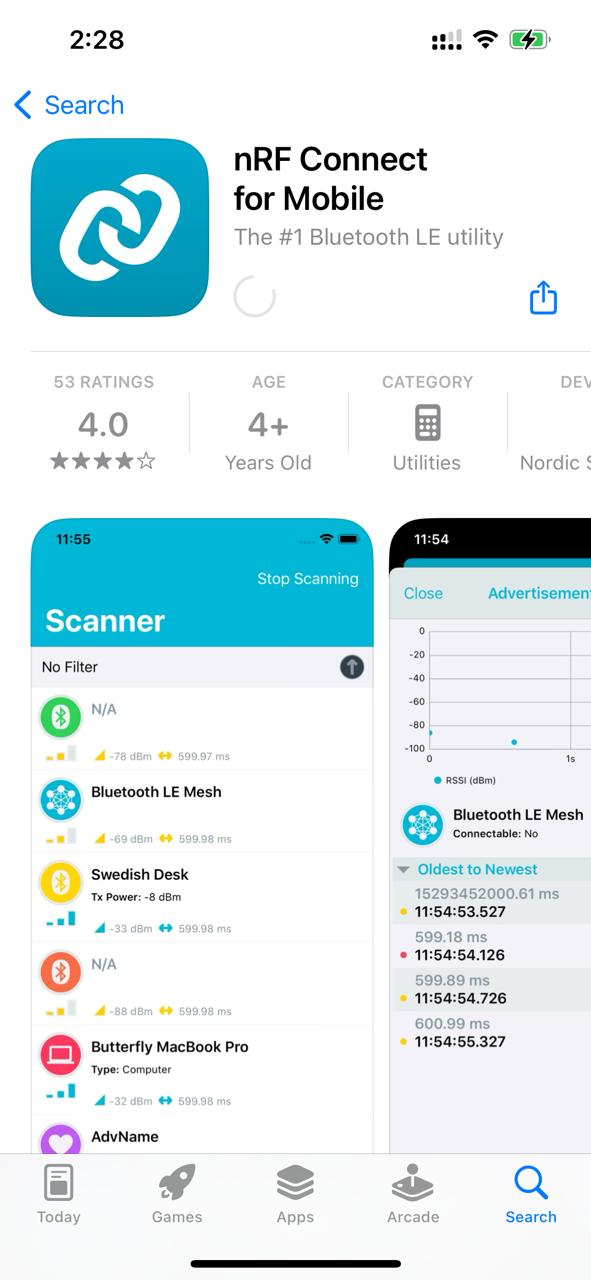
\includegraphics[width=0.7\linewidth]{Images/PortentaH7/NRF-Connect.jpg}
							\caption{NRF-Connect}
							\label{NRF-Connect}
						\end{center}
					\end{figure}
				Once you have downloaded the nRF application on your mobile device, look for your Portenta in the device list. You may filter the list by "Portenta" to easierly find your board in case you are using nRF Connect.
				
				\item When you find your board in the list tap "Connect".
				\item Navigate to the "Services" screen and tap the arrow up button.
				\item Switch to "Bool" type and move the toggle to "True". Confirm the dialog with a tap on "Write" and you should see the built-in LED turned on. If you do the same procedure again but setting the toggle switch to "False", it will turn off the LED. ~\ref{Bluetooth-scan}
					\begin{figure}
						\begin{center}
							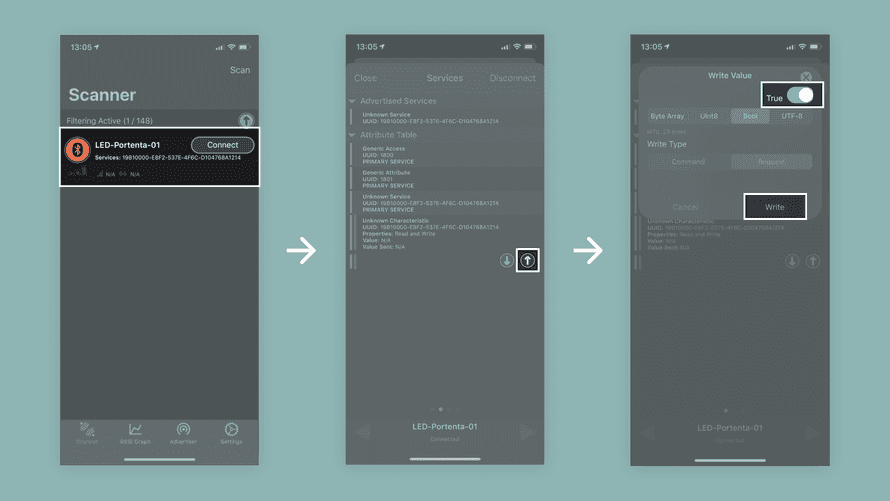
\includegraphics[width=0.7\linewidth]{Images/PortentaH7/Bluetooth-scan.png}
							\caption{Bluetooth-scan}
							\label{Bluetooth-scan}
						\end{center}
					\end{figure}
				\item \textbf{6. Conclusion:} This example shows how to connect and control the built-in LED using a Bluetooth® Low Energy connection. You have learned how a simple Bluetooth® Low Energy connection between your Portenta and your cell phone, which has basic communication abilities between the two devices, works. ~\ref{NRF-Connect}	
				
			\end{itemize}
		

		



\section{First Step with PortentaH7:}
	
	\subsection{Setting Up Portenta H7 For Arduino:}
		This Example teaches you how to set up the board, how to configure your computer and how to run the classic Arduino blink example to verify if the configuration was successful. ~\ref{PortentaH7-connection} \cite{portentaSetup:2024}
	\subsection{Goals:}
		\begin{itemize}
			\item About the Arduino and Mbed operating system (Mbed OS) stack
			\item Installing the Mbed library
			\item Controlling the built in LED on the Portenta board
		\end{itemize}
	\subsection{Instructions:}
		\begin{itemize}
			\item \textbf{Configuring the Development Environment:} In this section, we will guide you through a step-by-step process of setting up your Portenta board for running an Arduino Sketch that blinks the built-in RGB LED.
			\item \textbf{The Basic Setup:} Let's begin by Plug-in your Portenta to your computer using the appropriate USB-C® cable. Next, open your IDE and make sure that you have the right version of the Arduino IDE downloaded on to your computer.
				\begin{figure}
					\begin{center}
						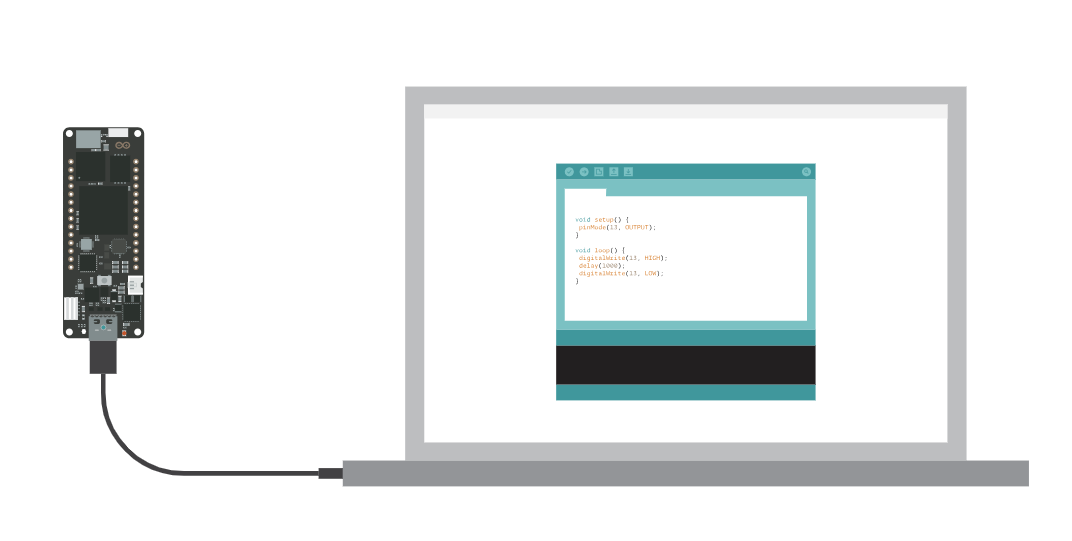
\includegraphics[width=0.7\linewidth]{Images/PortentaH7/PortentaH7-connection.png}
						\caption{PortentaH7-connection}
						\label{PortentaH7-connection}
					\end{center}
				\end{figure}
			\item \textbf{Adding the Portenta to the List of Available Boards:} In your Arduino IDE, open the board manager and search for "portenta". Find the Arduino mbed-enabled Boards library and click on "Install" to install the latest version of the mbed core (1.2.3 at the time of writing this tutorial). ~\ref{Portentaport}
				\begin{figure}
					\begin{center}
						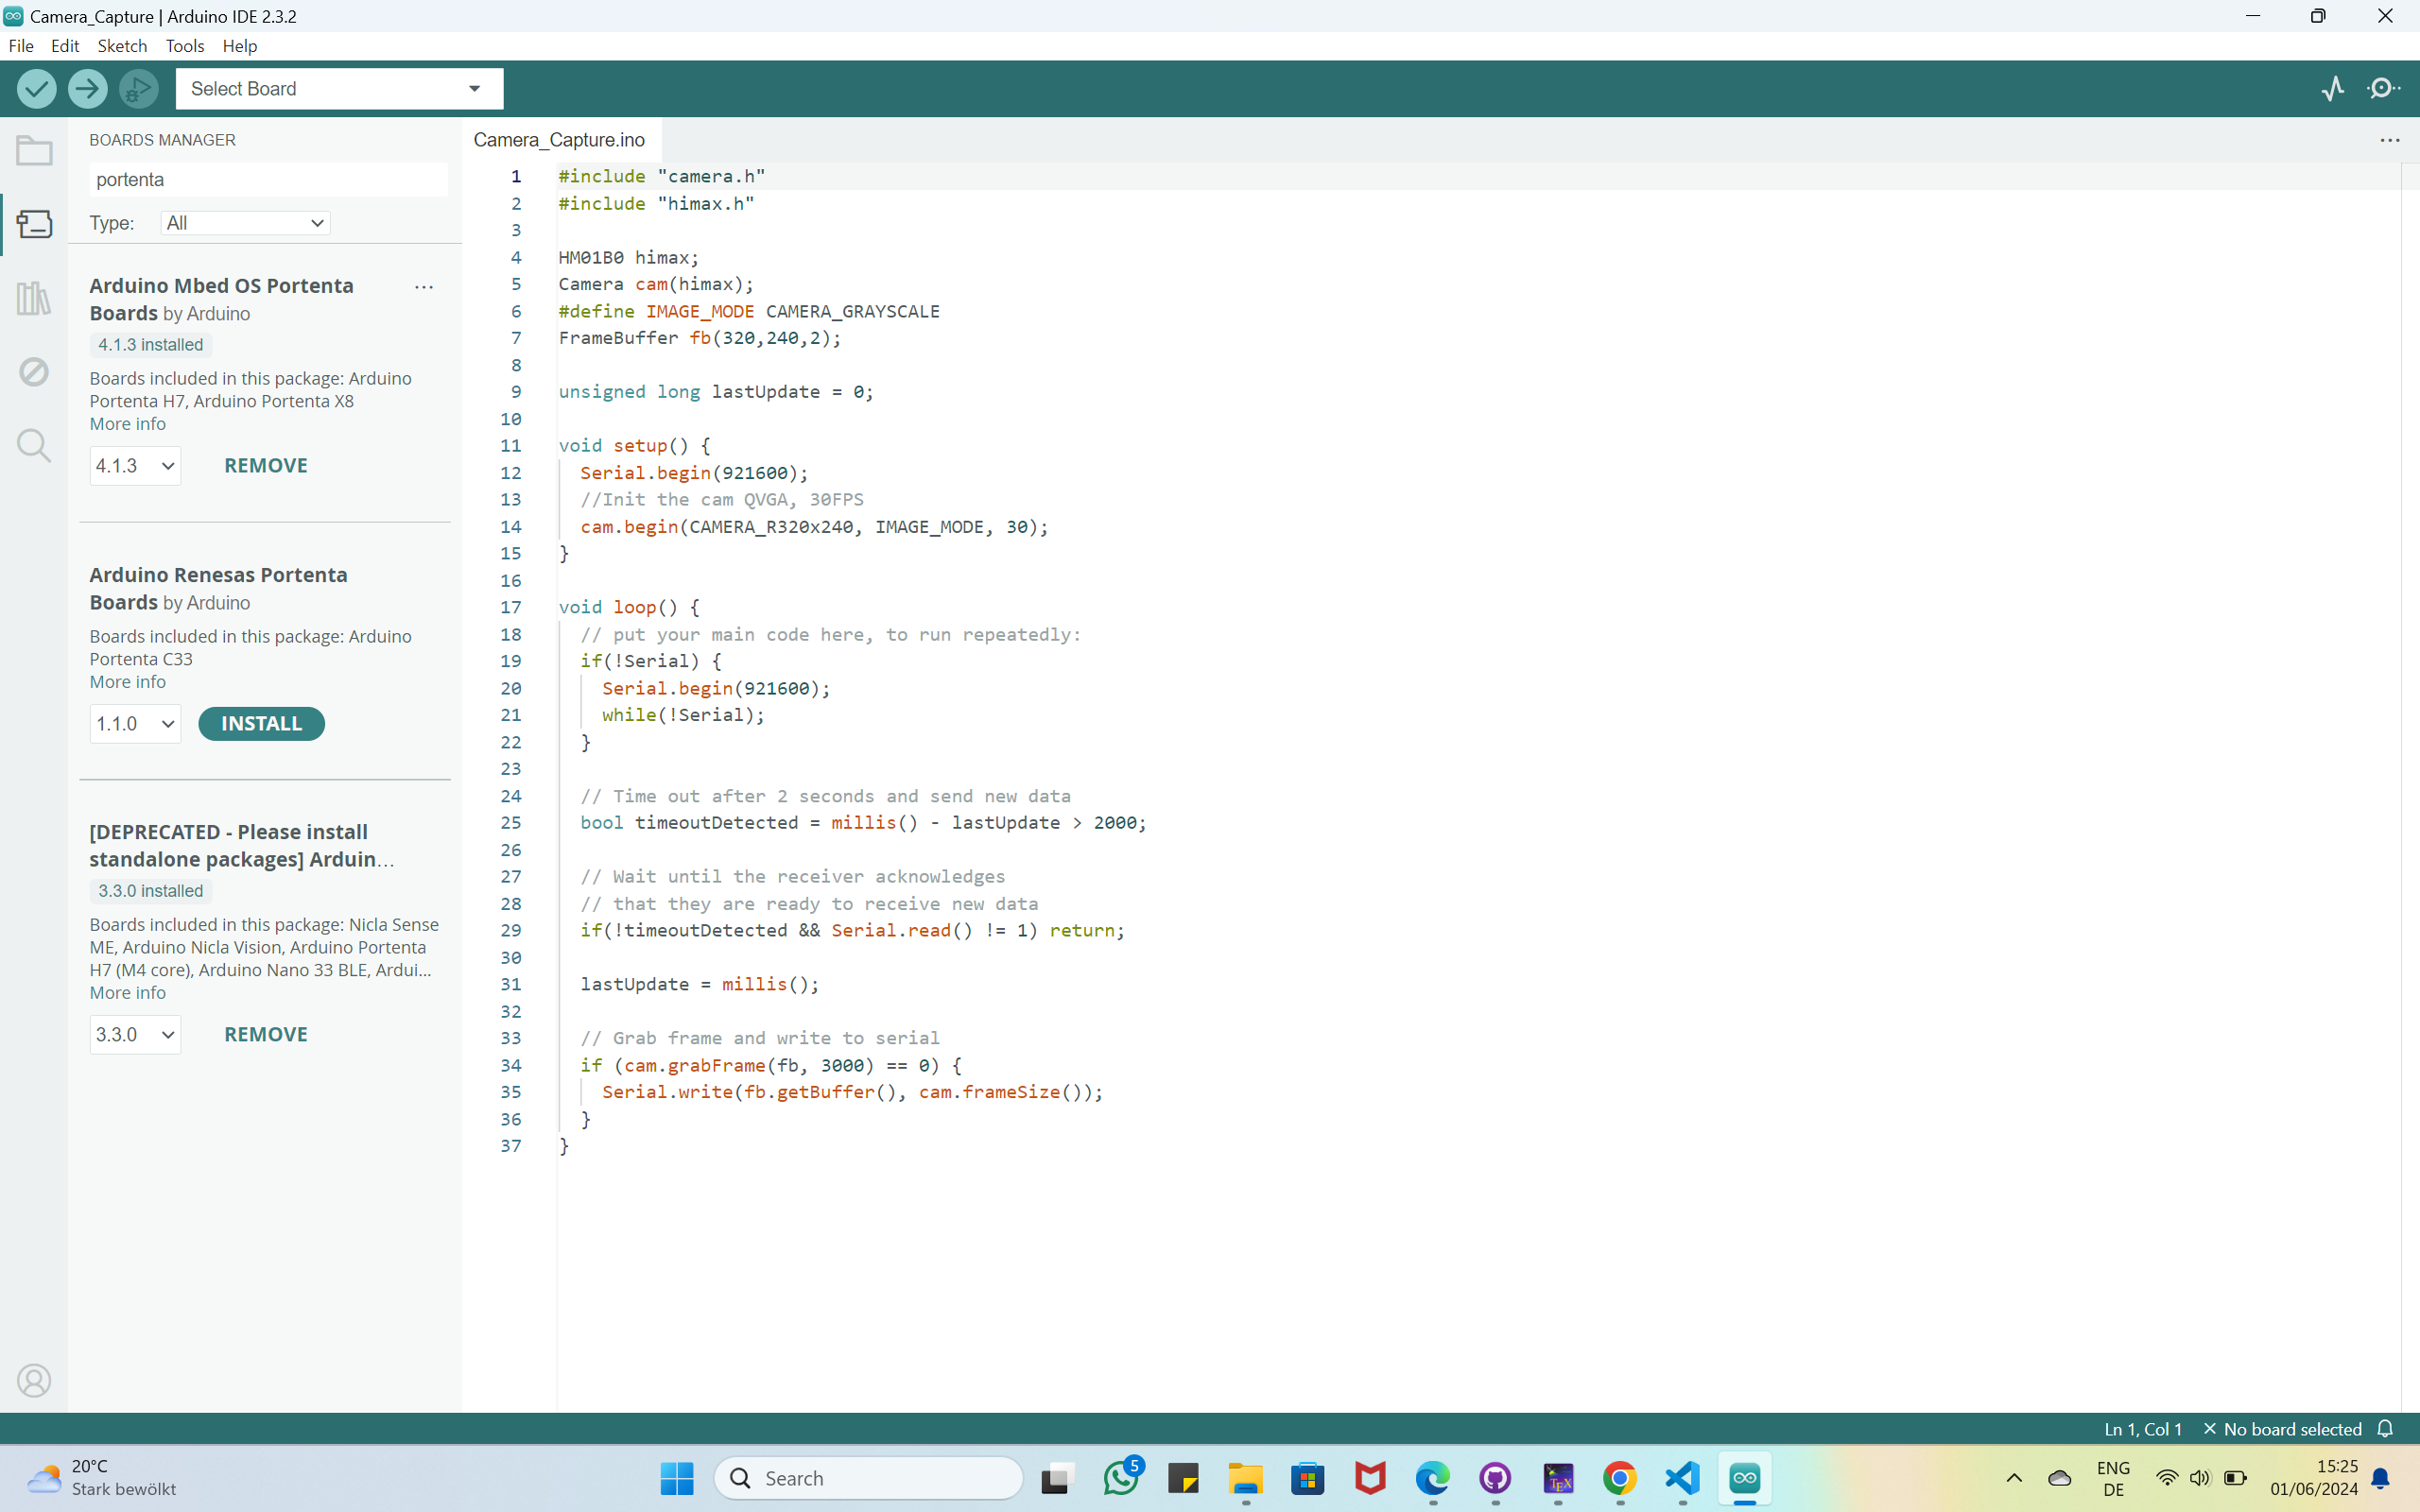
\includegraphics[width=0.7\linewidth]{Images/PortentaH7/Portentaport.png}
						\caption{Portentaport}
						\label{Portentaport}
					\end{center}
				\end{figure}
				
			\item \textbf{Uploading the Classic Blink Sketch:} Let's program the Portenta with the classic blink example to check if the connection to the board works. 
			
					\begin{lstlisting}
						// the setup function runs once when you press reset or power the board
						void setup() {
							// initialize digital pin LED_BUILTIN as an output.
							pinMode(LED_BUILTIN, OUTPUT);
							digitalWrite(LED_BUILTIN, HIGH); // turn the LED off after being turned on by pinMode()
						}
						
						// the loop function runs over and over again forever
						void loop() {
							digitalWrite(LED_BUILTIN, LOW); // turn the LED on (LOW is the voltage level)
							delay(1000); // wait for a second
							digitalWrite(LED_BUILTIN, HIGH); // turn the LED off by making the voltage HIGH
							delay(1000); // wait for a second
						}   
								
					\end{lstlisting}
			
		\end{itemize}
		
	\subsection{Conclusion:}
		You have now configured your Portenta board to run Arduino sketches. Along with that you gained an understanding of how the Arduino Core runs on top of Mbed OS.
		
		



